\documentclass[10pt,twocolumn,letterpaper]{article}

\usepackage{cvpr}
\usepackage{times}
\usepackage{epsfig}
\usepackage{graphicx}
\usepackage{amsmath}
\usepackage{amssymb}
\usepackage{subfigure}

% Include other packages here, before hyperref.

% If you comment hyperref and then uncomment it, you should delete
% egpaper.aux before re-running latex.  (Or just hit 'q' on the first latex
% run, let it finish, and you should be clear).
\usepackage[breaklinks=true,bookmarks=false]{hyperref}

\cvprfinalcopy % *** Uncomment this line for the final submission

\def\cvprPaperID{****} % *** Enter the CVPR Paper ID here
\def\httilde{\mbox{\tt\raisebox{-.5ex}{\symbol{126}}}}

% Pages are numbered in submission mode, and unnumbered in camera-ready
%\ifcvprfinal\pagestyle{empty}\fi
\setcounter{page}{4321}
\begin{document}

%%%%%%%%% TITLE
\title{Computer Vision Homework 3\\Implement Bag of visual words  and Spatial Pyramid Matching  method}

\author{Wencai Jiang\\
Shanghaitech University\\
{\tt\small jiangcw@shanghaitech.edu.cn}
% For a paper whose authors are all at the same institution,
% omit the following lines up until the closing ``}''.
% Additional authors and addresses can be added with ``\and'',
% just like the second author.
% To save space, use either the email address or home page, not both
}

\maketitle
%\thispagestyle{empty}

%%%%%%%%% ABSTRACT
\begin{abstract}
   This report introduces how to implement the algorithm for Recognizing Natural Scene Categories by Bag of visual words\cite{YANG2007Evaluating} and Spatial Pyramid Matching \cite{lazebnik2006beyond}. I test algorithm on the publicly available Caltech-256\cite{griffinHolubPerona}.
\end{abstract}

%%%%%%%%% BODY TEXT
\section{Introduction}
\subsection{Bag-of-Visual-Words}
Using image keypoints or local interest points in image retrieval and classification. Keypoints are salient image patches that contain rich local information of an image, and they can be automatically detected using various detectors  and represented by many descriptors [. Keypoints are then grouped into a large number of clusters so that those with similar descriptors are assigned into the same cluster. By treating each cluster as a “visual word” that represents the specific local pattern shared by the keypoints in that clus- ter, we have a visual-word vocabulary describing all kinds of local image patterns. With its keypoints mapped into vi- sual words, an image can be represented as a “bag of visual words”, or specifically, as a vector containing the (weighted) count of each visual word in that image, which can be used as a feature vector in classification task.
%-------------------------------------------------------------------------
\subsection{Spatial Pyramid Matching}
Although the Bags of Features has great performance, it is weak in spatial information. People can construct some strange images that consist of some of features without caring about the spatial structure, which can also be clas- sified as a targeted label with high probabil- ity. In this paper, the author proposed a new method that contain the spatial information, which called Spatial Pyramid Matching(SPM).
 
%------------------------------------------------------------------------
\section{Program analysis}
In this section we analyze the program step by step, and discuss the related parameters setting.\\
\subsection{Bag-of-Visual-Words}
 \indent we use the vector quantization (VQ) technique which clusters the keypoint descriptors in their feature space into a large number of clusters using the K-means clustering algorithm and encodes each keypoint by the index of the cluster to which it belongs. We conceive each cluster as a visual word that represents a specific lo- cal pattern shared by the keypoints in that cluster. Thus, the clustering process generates a visual-word vocabulary de- scribing different local patterns in images. The number of clusters determines the size of the vocabulary, which can vary from hundreds to over tens of thousands. By mapping the keypoints to visual words, we can represent each image as a “bag of visual words”. This representation is analo- gous to the bag-of-words document representation in terms of form and semantics. Both representations are sparse and high-dimensional, and just as words convey meanings of a document, visual words reveal local patterns characteristic of the whole image.
%-------------------------------------------------------------------------
\subsection{Spatial Pyramid Matching}
	 First,we need  to extract keypoints by SIFT and build codebook by KMean.For each RBG image, get gray image firstly and calculate the key points for $step size: 4$. Then, calculate the descriptors by key points. For all images, I got $X_train_feature$.\\
	 \par Set $K = 100$, use K-means to build codebook with $X_train_feature$.\\
	 \indent Then, Building Spatial Pyramid.Construct a sequence of grids at resolutions $l=0,1,2$, such that the grid at level $l$ has $2^l$ cells along each dimension, for a total of $D = 2^{dl}$ cells.、、
	 \indent Finally, for each level, concatenate the pyramid, and calculate the histogram with a weight.
%----------------------------------------------------------------------
\section{Result}
\subsection{Spectral Residual Approach}
\indent \indent  Here are the results of spectral residual approach shown in figure 1
\begin{figure}[h]
	\centering
	\subfigure[Original Image]{
		\fbox{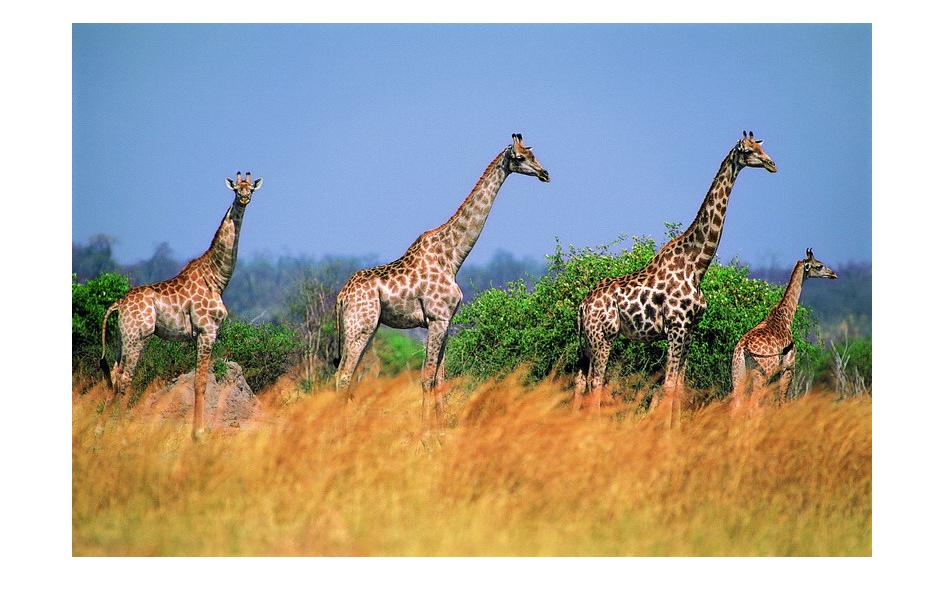
\includegraphics[width=3cm]{giraffe.jpg}}
	
		
	}
\subfigure[Saliency map]{

	\fbox{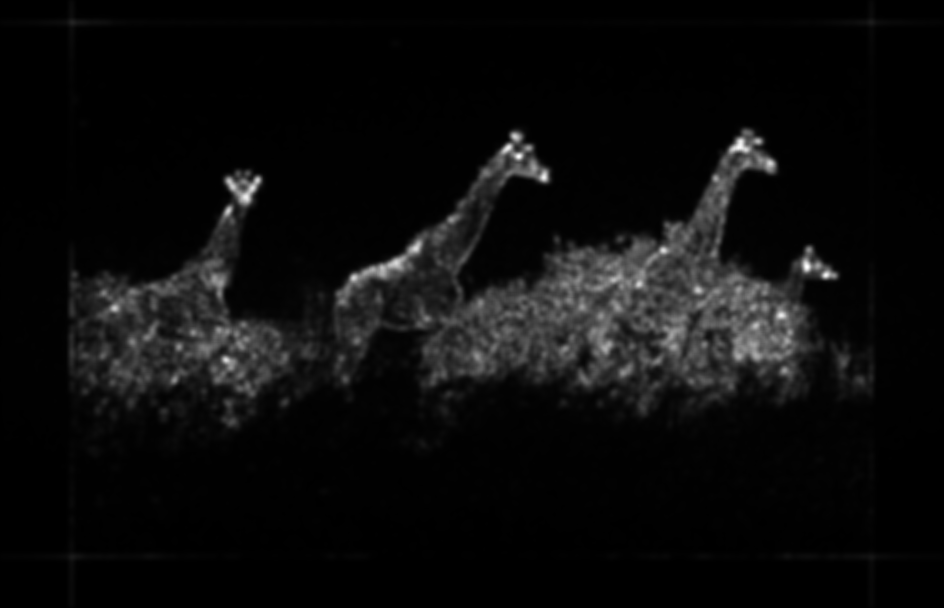
\includegraphics[width=3cm]{result.png}}
	
}
   \caption{ Left: input; Right: the result}
   
  
\end{figure}
 \subsection{Context-Aware Saliency Detection}
 First, Using the existing code on the Internet, I try to divide the picture into different number of super pixels,the image segmentation results shown in Figure 2.\\

 \begin{figure}[h]
	\centering
 	\subfigure[Original Image]{
 		\centering
 		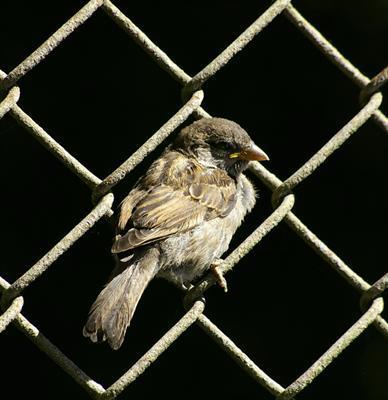
\includegraphics[width=3cm]{result/bird.jpg}

 
}
\subfigure[200 pieces]{
	\centering
	
	
\includegraphics[width=3cm]{result/200.png}
	
}
 		\subfigure[400 pieces]{
 			\centering
 			
\includegraphics[width=3cm]{result/400.png}
 	
 			
 		}
 		\subfigure[800 pieces]{
 			\centering
 		
 			
\includegraphics[width=3cm]{result/800.png}
 			
 		}
 	\caption{ Image split into 200、400 and 800 pieces}
 	
 	
 \end{figure}
 
 \indent \indent Then I use 4 scales in the program to calculate the saliency:$R = r, \frac{1}{2}r, \frac{1}{4}r, \frac{1}{8}r$. Saliency of patches under different
 scales are shown in Figure 3.
 
 \begin{figure}[h]
 	\centering
 	\subfigure[scale=r]{
 		\centering
 		
\includegraphics[width=3cm]{result/1.png}
 		
 		
 	}
 	\subfigure[scale=r/2]{
 		\centering
 		
 		
\includegraphics[width=3cm]{result/2.png}
 		
 	}
 	\subfigure[scale=r/4]{
 		\centering
 		
\includegraphics[width=3cm]{result/4.png}
 		
 		
 	}
 	\subfigure[scale=r/8]{
 		\centering
 		
 		
\includegraphics[width=3cm]{result/8.png}
 		
 	}
 	\caption{Saliency of patches under different
 		scales}
 	
 	
 \end{figure}
 
 
 \indent \indent Finally,Taking the mean of the saliency at pixel $i$ at different scales and giving pixel saliency weight according to their distance to the foci to get the final computed saliency . The results shown in Figure 4.
 \begin{figure}[h]
 	\centering
 	\subfigure[mean pixel]{
 		\centering
 		
\includegraphics[width=3cm]{result/mean_S_pixel.png}
 		
 		
 	}
 	\subfigure[weighted pixe]{
 		\centering
 		
 		
\includegraphics[width=3cm]{result/weighted_S_pixel.png}
 		
 	}
 
 	\caption{Taking the mean of the saliency at pixel $i$ and giving pixel saliency weight }
 	
 	
 \end{figure}


{\small
\bibliographystyle{ieee}
\bibliography{reference.bib}
}

\end{document}
